\documentclass[border=1cm]{standalone}
\usepackage{tikz}
\usetikzlibrary{shapes.geometric, arrows, positioning}

% Estilos
\tikzstyle{startstop} = [
    rectangle, rounded corners, minimum width=3.7cm, minimum height=1.5cm, 
    text centered, align=center, draw=black, fill=red!30
]
\tikzstyle{process} = [
    rectangle, minimum width=3.7cm, minimum height=1.5cm, 
    text centered, align=center, draw=black, fill=orange!30
]
\tikzstyle{arrow} = [thick,->,>=stealth]

\begin{document}
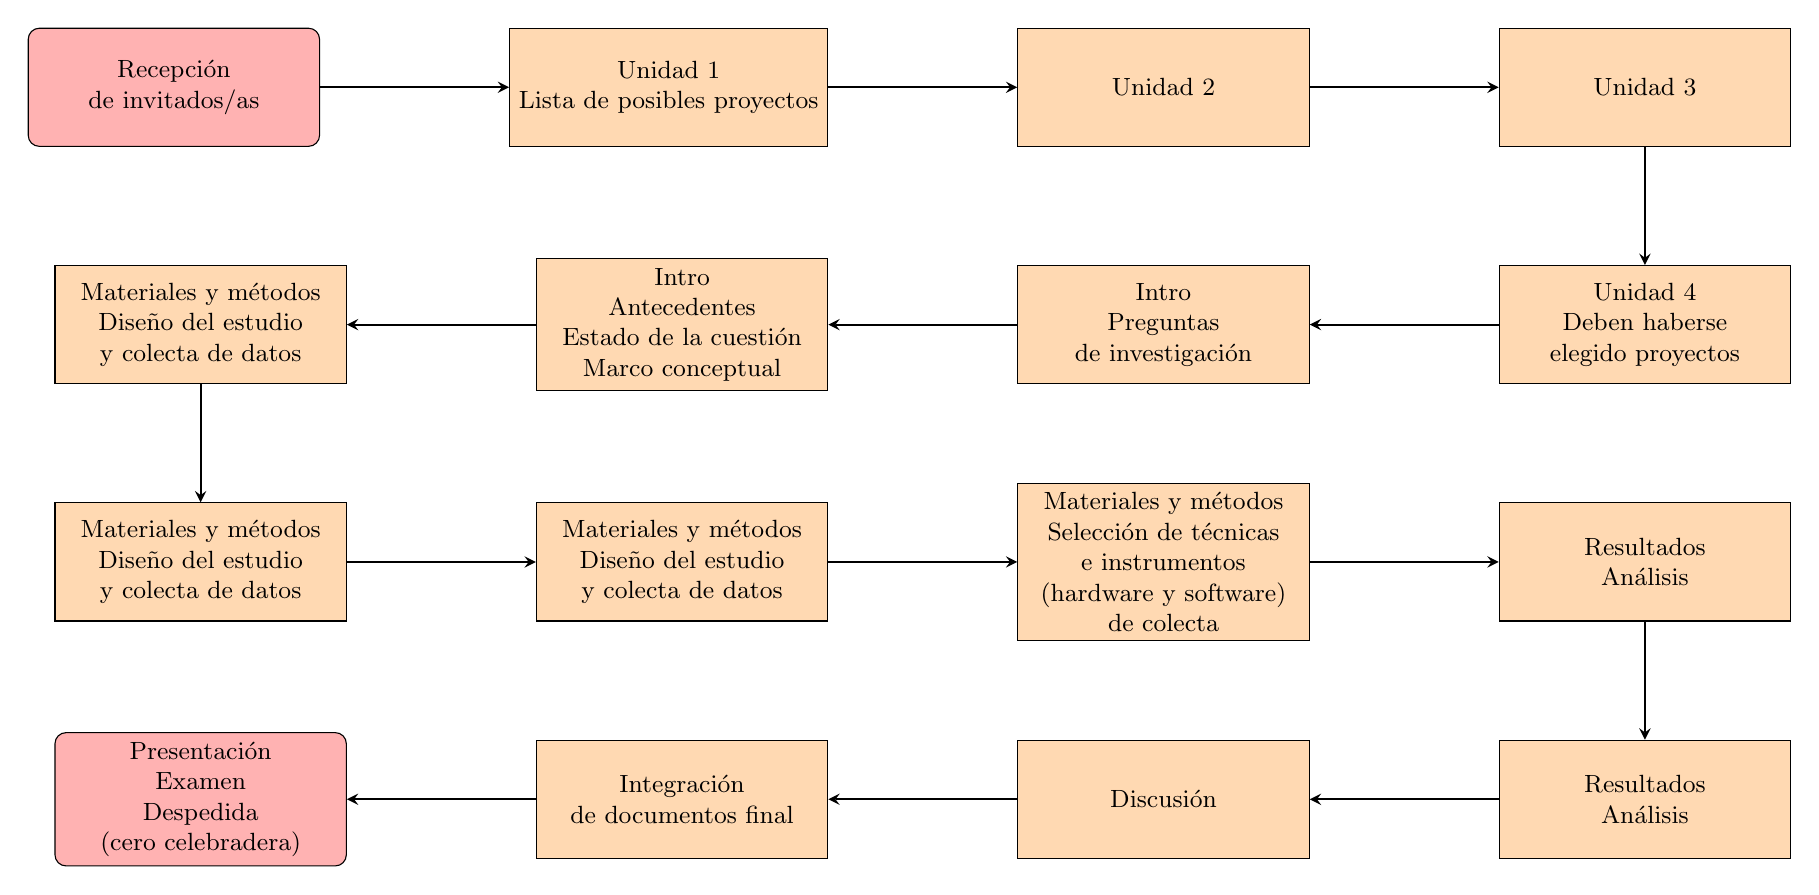
\begin{tikzpicture}[
    node distance=1.5cm and 2.4cm,
    font=\small
]

% Fila 1 (izquierda a derecha)
\node (n0)  [startstop]                                   {Recepción \\ de invitados/as};
\node (n1)  [process, right=of n0]                        {Unidad 1 \\ Lista de posibles proyectos};
\node (n2)  [process, right=of n1]                        {Unidad 2};
\node (n3)  [process, right=of n2]                        {Unidad 3};

% Fila 2 (derecha a izquierda)
\node (n4)  [process, below=of n3]                        {Unidad 4 \\ Deben haberse \\ elegido proyectos};
\node (n5)  [process, left=of n4]                         {Intro \\ Preguntas \\ de investigación};
\node (n6)  [process, left=of n5]                         {Intro \\ Antecedentes \\ Estado de la cuestión \\ Marco conceptual};
\node (n7)  [process, left=of n6]                         {Materiales y métodos \\ Diseño del estudio \\ y colecta de datos};

% Fila 3 (izquierda a derecha)
\node (n8)  [process, below=of n7]                        {Materiales y métodos \\ Diseño del estudio \\ y colecta de datos};
\node (n9)  [process, right=of n8]                        {Materiales y métodos \\ Diseño del estudio \\ y colecta de datos};
\node (n10) [process, right=of n9]                        {Materiales y métodos \\ Selección de técnicas \\ e instrumentos \\ (hardware y software) \\ de colecta};
\node (n11) [process, right=of n10]                       {Resultados \\ Análisis};

% Fila 4 (derecha a izquierda)
\node (n12) [process, below=of n11]                       {Resultados \\ Análisis};
\node (n13) [process, left=of n12]                        {Discusión};
\node (n14) [process, left=of n13]                        {Integración \\ de documentos final};
\node (n15) [startstop, left=of n14]                      {Presentación \\ Examen \\ Despedida \\
(cero celebradera)};

% Flechas (zigzag)
\draw [arrow] (n0) -- (n1);
\draw [arrow] (n1) -- (n2);
\draw [arrow] (n2) -- (n3);
\draw [arrow] (n3) -- (n4);
\draw [arrow] (n4) -- (n5);
\draw [arrow] (n5) -- (n6);
\draw [arrow] (n6) -- (n7);
\draw [arrow] (n7) -- (n8);
\draw [arrow] (n8) -- (n9);
\draw [arrow] (n9) -- (n10);
\draw [arrow] (n10) -- (n11);
\draw [arrow] (n11) -- (n12);
\draw [arrow] (n12) -- (n13);
\draw [arrow] (n13) -- (n14);
\draw [arrow] (n14) -- (n15);

\end{tikzpicture}
\end{document}
